\chapter{Planificación}

\noindent\fbox{
	\parbox{\textwidth}{
		En este capítulo realizaremos una estimación del tiempo necesario para realizar el proyecto, y cuantificaremos las tareas que se deberían cumplir, acabando con un diagrama de Gantt que contará gráficamente el tiempo empleado en realizarlos aproximadamente.
	}
}

\section{Metodología utilizada}
Para desarrollar el proyecto se ha optado por una Metodología Ágil basada en SCRUM, ya que permite mucha flexibilidad temporal y mayor control en las tareas que hay que realizar. Además, si hay alguna tarea que se debe añadir durante el desarrollo, se puede introducir al backlog y tratarlo posteriormente.

\section{Temporización}
A grandes rasgos, se han desarrollado los objetivos separándolos en acciones más pequeñas para poder cumplirlas. En el análisis se terminarán de definir todas las tareas con tal de poder tener un Product Backlog definido totalmente para poder desarrollar todo lo necesario.

\subsection{El Product Backlog}

Aparte de los requisitos ya especificados en el apartado anterior, tendremos que añadir una parte de análisis donde, además de realizar diagramas para plasmar la idea a algo tangible:

\begin{itemize}
	\item Compararemos las distintas APIs de Reconocimiento de Voz
	\item Compararemos las distintas APIs de Síntesis de Voz
\end{itemize}

Por otra parte, habrá que incluir de cara a la puesta a publicación de este proyecto una serie de documentos y extras:

\begin{itemize}
	\item Realización de un Readme para explicar qué es y cómo funciona
	\item Realización de una Guía de contribución para estandarizar una manera de compartir las maneras de solventar fallos.
	\item Aplicación de la licencia al proyecto, según lo comentado en el Objetivo O-IA 6.
\end{itemize}

Por tanto, el Product Backlog se listaría de la siguiente forma:

\begin{center}
		\begin{xltabular}{\textwidth}{|c|c|X|c|}
			\hline
			{\cellcolor{mintgreen}} \textbf{Nº ID} & {\cellcolor{mintgreen}} \textbf{Refiere a\newline (RF/Otro)} & {\cellcolor{mintgreen}} \textbf{Descripción} & {\cellcolor{mintgreen}} \textbf{Prioridad} \\
			\hline
			1 & RF-1. & Hablar al Asistente & Alta \\
			\hline
			2 & RF-2. & Escuchar una respuesta del Asistente & Alta \\
			\hline
			3 & RF-3. & Sintetizar la voz de una pregunta en un texto & Alta \\
			\hline
			4 & RF-4. & Generar un audio leyendo una respuesta & Alta \\
			\hline
			5 & RF-5. & Relacionar una pregunta con su respuesta & Alta \\
			\hline
			6 & Otro & Comparar las APIs de Reconocimiento de Voz & Alta \\
			\hline
			7 & Otro & Comparar las APIs de Síntesis de Voz & Alta \\
			\hline
			8 & RF-6. & Avisar de que no se puede conectar a Internet & Media \\
			\hline
			9 & RF-7. & Responder que se desconoce la respuesta a una pregunta & Media \\
			\hline
			10 & Otro & Aplicar la Licencia al proyecto & Media \\
			\hline
			11 & Otro & Crear un README para explicar cómo instalar y usar el proyecto & Media \\
			\hline
			12 & Otro & Crear una Guía de Conducta para explicar cómo realizar contribuciones al proyecto & Baja \\
			\hline
			\caption{Product Backlog del proyecto en la planificación inicial.}
		\end{xltabular}
\end{center}

\subsection{División en sprints}
Un primer esbozo para dividir todas las tareas en 3 grandes sprints de forma que se vayan realizando de forma continua y constante.

\subsubsection{Sprint 0: Análisis, comparación y planteamiento del sistema ( 4 semanas)}
En este primer sprint se preparará todo lo necesario para empezar a programar el sistema.

Por una parte, trataremos de resolver estos puntos del Backlog:

\begin{table}[H]
	\begin{tabularx}{\textwidth}{|c|X|c|}
		\hline
		{\cellcolor{mintgreen}} \textbf{Nº ID} & {\cellcolor{mintgreen}} \textbf{Descripción} & {\cellcolor{mintgreen}} \textbf{Prioridad} \\
		\hline
		6 &  Comparar las APIs de Reconocimiento de Voz & Alta \\
		\hline
		7 &  Comparar las APIs de Síntesis de Voz & Alta \\
		\hline
	\end{tabularx}
\end{table}

Por otra parte, se realizarán los diagramas necesarios para poder cumplir los requisitos establecidos.

\subsubsection{Sprint 1: Adaptando las APIs al proyecto (2 semanas)}
En este primer Sprint se trasteará con las librerías seleccionadas para poder adaptar sus métodos y así simplificar las llamadas a estas en base a lo planeado en el análisis.

Trataremos de resolver los siguientes puntos del Backlog:

\begin{table}[H]
	\begin{tabularx}{\textwidth}{|c|X|c|}
		\hline
		{\cellcolor{mintgreen}} \textbf{Nº ID} & {\cellcolor{mintgreen}} \textbf{Descripción} & {\cellcolor{mintgreen}} \textbf{Prioridad} \\
		\hline
		1 & RF-1. Hablar al Asistente & Alta \\
		\hline
		2 & RF-2. Escuchar una respuesta del Asistente & Alta \\
		\hline
		3 & RF-3. Sintetizar la voz de una pregunta en un texto & Alta \\
		\hline
		4 & RF-4. Generar un audio leyendo una respuesta & Alta \\
		\hline
	\end{tabularx}
\end{table}

\subsubsection{Sprint 2: Conectando preguntas con respuestas (6 semanas)}
El segundo Sprint es el más importante del proyecto, ya que nos permitirá completar todo el flujo de funcionamiento del Asistente gracias a que podrá saber qué pregunta se formula y buscar si puede dar una respuesta.

Trataremos de resolver los siguientes puntos del Backlog del producto:
\begin{table}[H]
	\begin{tabularx}{\textwidth}{|c|X|c|}
		\hline
		{\cellcolor{mintgreen}} \textbf{Nº ID} & {\cellcolor{mintgreen}} \textbf{Descripción} & {\cellcolor{mintgreen}} \textbf{Prioridad} \\
		\hline
			5 & RF-5. Relacionar una pregunta con su respuesta & Alta \\
		\hline
			9 & RF-7. Responder que se desconoce la respuesta a una pregunta & Media \\
		\hline
	\end{tabularx}
\end{table}

\subsubsection{Sprint 3: Haciendo algunas funcionalidades de muestra al Asistente ( 4 semanas)}

En este punto, tenemos un Asistente que podría escuchar y hablar, pero no sabe qué responder ante cualquier cosa que le preguntemos. Por lo tanto, hay que darle algunos conocimientos con algunas funcionalidades de muestra.

Trataremos de resolver los siguientes puntos del Backlog:
\begin{table}[H]
	\begin{tabularx}{\textwidth}{|c|X|c|}
		\hline
		{\cellcolor{mintgreen}} \textbf{Nº ID} & {\cellcolor{mintgreen}} \textbf{Descripción} & {\cellcolor{mintgreen}} \textbf{Prioridad} \\
		\hline
			8 & RF-6. Avisar de que no se puede conectar a Internet & Media \\
		\hline
	\end{tabularx}
\end{table}

Además de ello, se tendrían que crear algunas funcionalidades (dentro del tiempo que nos ocupa) para poder presentar el producto con algo a lo que pueda responder.

\subsubsection{Sprint 4: Adaptando el repositorio para su liberación (2 semanas)}

En la recta final del trabajo, antes de entregar el proyecto para la evaluación y de poder liberarse el repositorio, necesitaremos preparar algunas instrucciones para que cualquiera lo pueda probar y modificar a su antojo.

Se probaría a resolver estos puntos del Backlog:
\begin{table}[H]
	\begin{tabularx}{\textwidth}{|c|X|c|}
		\hline
		{\cellcolor{mintgreen}} \textbf{Nº ID} & {\cellcolor{mintgreen}} \textbf{Descripción} & {\cellcolor{mintgreen}} \textbf{Prioridad} \\
		\hline
		10 &  Aplicar la Licencia al proyecto & Media \\
		\hline
		11 & Crear un README para explicar cómo instalar y usar el proyecto & Media \\
		\hline
		12 & Crear una Guía de Conducta para explicar cómo realizar contribuciones al proyecto & Baja \\
		\hline
	\end{tabularx}
\end{table}

En este punto, habrá también que comprobar que el sistema en su conjunto funcione, lo que se podría alargar por temas de debugging y pruebas.

\subsection{Velocidad de equipo}
En términos de Velocidad, habría que considerar que cada día que se dedica a este proyecto tiene una media de 3 horas y 30 minutos.

Hay 4 días de media a la semana donde se puede dedicar a la realización del Asistente. 

En total, cada semana se trabajaría una media de 14 horas a partir de la Fase de Análisis.

Al ser 20 semanas, se estiman un total de 280 horas totales dedicadas al proyecto en total a partir de la fase de análisis. (56 horas en el Sprint 0, 28 en el Sprint 1, 84 en el Sprint 2, y 56 horas por cada uno de los Sprints restantes)

\subsection{Diagrama de Gantt}
La temporización en este punto quedaría desarrollada por el Diagrama de Gantt ubicada en la Figura \ref{fig:gantt} en la página \pageref{fig:gantt}

\begin{figure}[h]
	\centering
	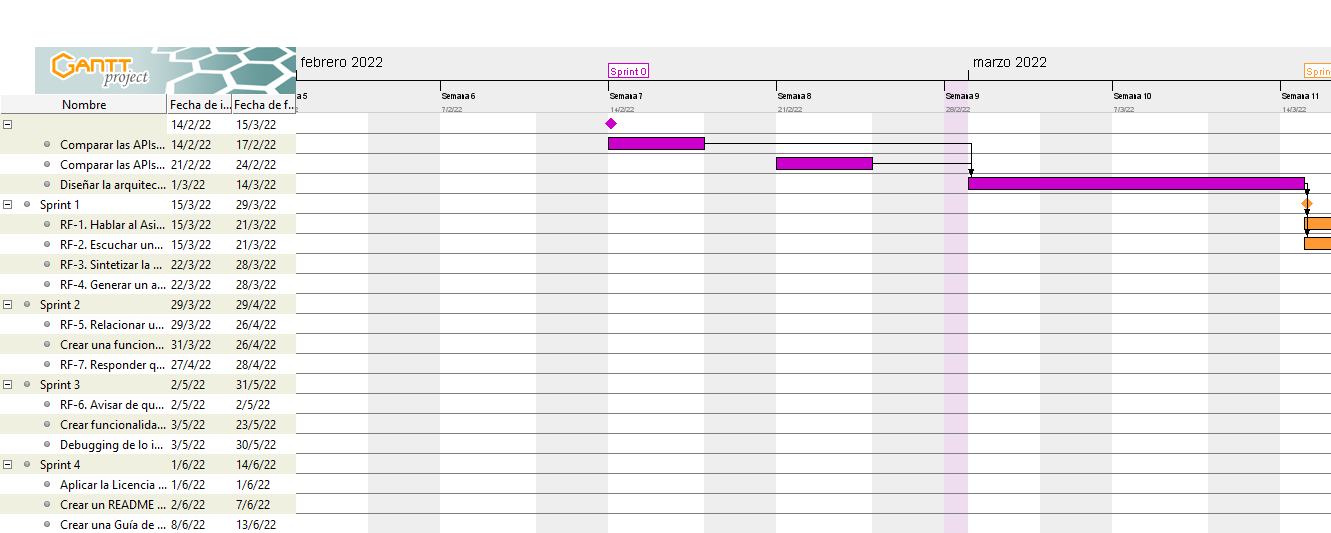
\includegraphics[width=\textwidth]{imagenes/Gantt1.png} \\
	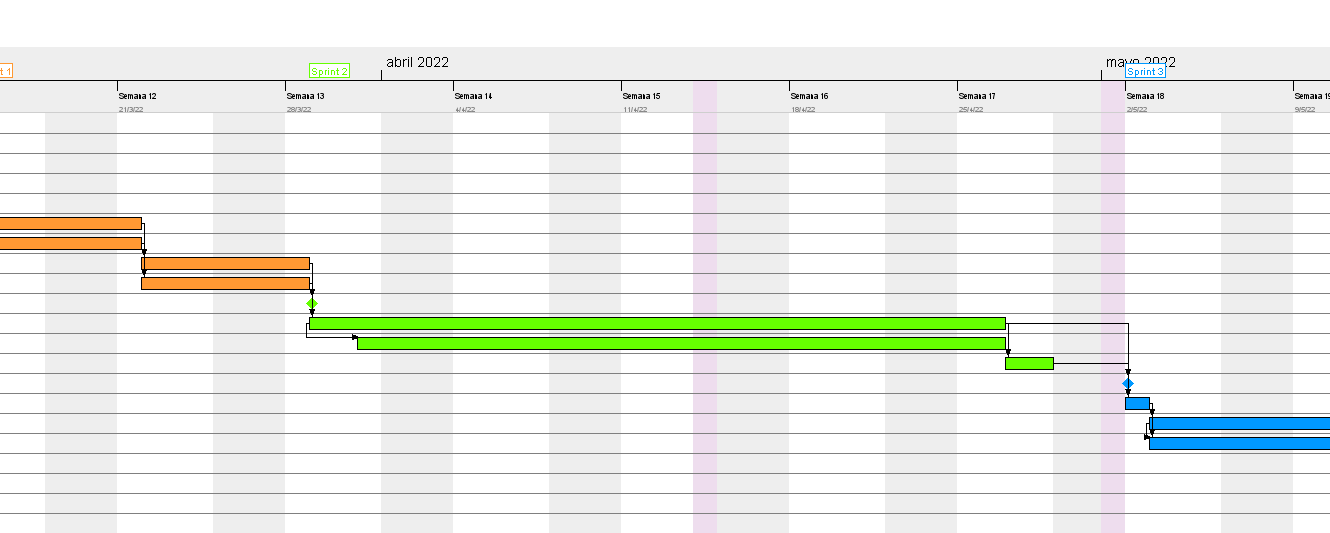
\includegraphics[width=\textwidth]{imagenes/Gantt2.png} \\
	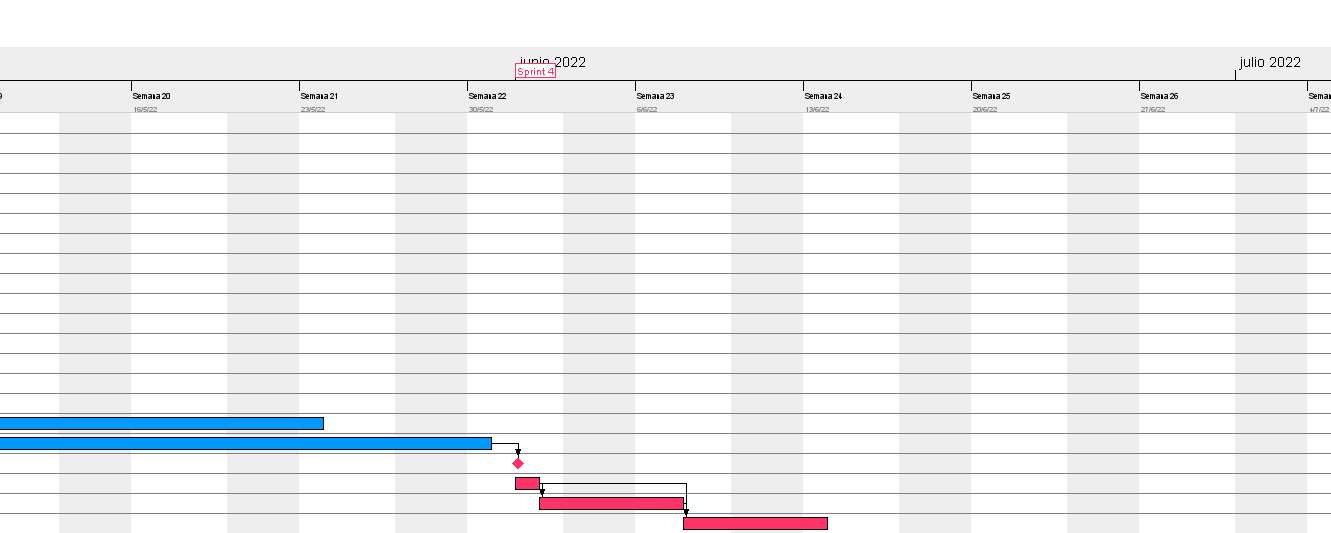
\includegraphics[width=\textwidth]{imagenes/Gantt3.png} \\
	\caption[Diagrama de Gantt]{Diagrama de Gantt del proyecto. De elaboración propia, generado con GanttProject.}
	\label{fig:gantt}
\end{figure}


\section{Seguimiento del desarrollo}
Para seguir el desarrollo se hará uso de dos artefactos que acompañan al framework SCRUM \cite{scrum}:
\begin{itemize}
	\item Sprint Backlogs : Al principio de cada Sprint se revisará si queda alguna tarea pendiente y si hay que recalcular algo. Como base tendremos los de la subsección 5.2.1
	\item Gráfica de Burndown: Cada vez que se termine una tarea se actualizará esta gráfica.
\end{itemize}

\section{Estimación de costes}
\subsection{El personal}
Si bien este proyecto se va a acabar realizando por una persona realmente, supongamos el caso de que este proyecto lo realizara una pequeña startup de 4 miembros, de forma que hubiera un Scrum Master, un Product Owner, un documentalista y un desarrollador que trabajará principalmente en Python.

Para el Sprint 0, estimaremos las horas que harían cada uno en base a estos porcentajes:
\begin{itemize}
	\item \textbf{Programador}: 50\% \textrightarrow 28 h
	\item \textbf{Documentalista}: 30\% \textrightarrow 16'8 h
	\item \textbf{Product Owner}: 15\% \textrightarrow 8'4 h
	\item \textbf{Scrum Master}: 5\% \textrightarrow 2'8 h
\end{itemize}

En los Sprints 1 al 3, seguirán estos porcentajes:
\begin{itemize}
	\item \textbf{Programador}: 70\% \textrightarrow 19'6 h (Sp. 1) / 58'8 h (Sp. 2)/ 39'2 h (Sp. 3)
	\item \textbf{Documentalista}: 10\% \textrightarrow 2'8 h (Sp. 1)/ 8'4 h (Sp. 2)/ 5'6 h (Sp. 3)
	\item \textbf{Product Owner}: 10\% \textrightarrow 2'8 h (Sp. 1)/ 8'4 h (Sp. 2)/ 5'6 h (Sp. 3)
	\item \textbf{Scrum Master}: 10\% \textrightarrow 2'8 h (Sp. 1)/ 8'4 h (Sp. 2)/ 5'6 h (Sp. 3)
\end{itemize}

Para el Sprint 4, estos serían los porcentajes estimados:
\begin{itemize}
	\item \textbf{Programador}: 50\% \textrightarrow 28 h
	\item \textbf{Documentalista}: 40\% \textrightarrow 22'4 h
	\item \textbf{Product Owner}: 5\% \textrightarrow 2'8 h
	\item \textbf{Scrum Master}: 5\% \textrightarrow 2'8 h
\end{itemize}

Por otra parte, se han comprobado los sueldos medios anuales para los siguientes cargos. Se ha tratado de localizar estos sueldos en el entorno de Granada (el único del que no se tenía información dedicada fue para el cargo de documentalista) La información fue obtenida a través de la plataforma Glassdoor, donde a partir de los datos que entregan trabajadores sobre sus empresas, hacen estadísticas sobre las empresas y los puestos.

Para hacer la conversión a horas, se ha supuesto un trabajo de 40 horas semanales.
\begin{itemize}
	\item \textbf{Programador} \cite{glassdoor-softwaredeveloper}: 24995 €/año \textrightarrow 12'02 €/hora
	\item \textbf{Documentalista} \cite{glassdoor-documentalist}: 46311,54 €/año \textrightarrow 22'27 €/hora
	\item \textbf{Product Owner} \cite{glassdoor-productowner}: 34844 €/año \textrightarrow 16'75 €/hora
	\item \textbf{Scrum Master} \cite{glassdoor-ScrumMaster}: 31682 €/año \textrightarrow 15'23 €/hora
\end{itemize}

\begin{center}
	\begin{table}[H]
		\centering
		\begin{tabularx}{\textwidth}{|X|X|X|X|}
			\hhline{|-|-|-|-|}
			{\cellcolor{lightblue}} \textbf{Trabajador} & {\cellcolor{lightblue}} \textbf{Tiempo dedicado (horas)} & {\cellcolor{lightblue}} \textbf{Coste por hora (€)} & {\cellcolor{lightblue}} \textbf{Total (€)} \\
			\hline
			Programador Python & 173'6 & 12'02 & 2.086'68  \\
			\hline
			Documentalista & 56 & 22'27 & 1.247'12 \\
			\hline
			Scrum Master & 22'4 & 16'75 & 375'2 \\
			\hline
			Product Owner & 28 & 15'23 & 426'44 \\
			\hline
			\textbf{Total} & \textbf{280} & - & \textbf{4.135'43} \\
			\hline
		\end{tabularx}
		\caption{Tabla de estimación de costes por personal}
	\end{table}
\end{center}
	
\subsection {Costes de productos físicos}
En el inventario hardware del proyecto se usarían dos dispositivos principalmente: Un ordenador portátil donde se desarrolle y pruebe el proyecto, y una Raspberry Pi 3B para las pruebas que se quieran hacer.

Listamos en la siguiente tabla los costes relacionados con ellos:

\begin{center}
	\begin{table}[H]
		\centering
		\begin{tabularx}{\textwidth}{|X|X|X|X|X|}
			\hline
			{\cellcolor{lightblue}}\textbf{Producto} & 
			{\cellcolor{lightblue}}\textbf{Vida útil (años)} &  {\cellcolor{lightblue}}\textbf{Coste (€)} &
			{\cellcolor{lightblue}}\textbf{Tiempo de implicación en el proyecto (meses)} &
			{\cellcolor{lightblue}}\textbf{Coste por uso (€)} \\
			\hline
			Raspberry Pi 3B & 8 & 35 & 1 & 0'36\\
			\hline
			Portátil HP Pavilion Gaming 15-2008ec & 4 & 550 & 5 & 57'29\\
			\hline
		\end{tabularx}
		\caption{Tabla de estimación de costes por productos físicos}
	\end{table}
\end{center}
\vfill

\subsection{Costes de productos lógicos}
En el caso de las herramientas software, notamos que todas son gratuitas, pero debido a que son unas cuantas y con propósitos variados, vemos interesante desglosarlos.

\begin{center}
	\begin{table}[H]
		\centering
		\begin{tabularx}{\textwidth}{|l|X|X|}
			\hline
			{\cellcolor{lightblue}}\textbf{Producto} & {\cellcolor{lightblue}}\textbf{Descripción} & {\cellcolor{lightblue}}\textbf{Coste (en €)} \\
			\hline
			Visual Studio Code & Editor de Código. Soporta integraciones para Python, entre otros lenguajes & 0 \\
			\hline
			Vosk/Mozilla Deepspeech & Framework de Código Abierto para Reconocimiento de Voz & 0 \\
			\hline
			eSpeak / Festival & Framework de Código Abierto para Text-to-Speech & 0 \\
			\hline
			PyAudio & Librería para gestionar la grabación y reproducción de audio & 0 \\
			\hline
			TeX Studio & Editor de \LaTeX  para redactar la documentación & 0 \\
			\hline
			Draw.io & Editor de Diagramas en la nube & 0 \\
			\hline
			GitHub & Almacén para el repositorio, basado en Git. La visibilidad privada está integrada en el \textit{Students Pack} & 0 \\
			\hline
			GanttProject & Editor de Diagramas de Gantt & 0 \\
			\hline
			Kubuntu 20.04 & Sistema Operativo para PCs x86 & 0 \\
			\hline
			Raspberry Pi OS  & Sistema Operativo para PCs ARM (como Raspberry Pi) & 0 \\
			\hline
			& \textbf{Total} & \textbf{0} \\
			\hline
		\end{tabularx}
		\caption{Tabla de estimación de costes por productos lógicos}
	\end{table}
\end{center}

%\newpage

\subsection{Presupuesto total}
En total, nos daríamos con el siguiente presupuesto:

\begin{center}
	\begin{table}[H]
		\centering
		\begin{tabularx}{10cm}{|X|X|}
			\hline
			{\cellcolor{lightblue}}\textbf{Concepto} & {\cellcolor{lightblue}}\textbf{Total (€)}  \\
			\hline
			Personal & 4.135'43 \\
			\hline
			Productos físicos & 57'65 \\
			\hline
			Productos lógicos & 0\\
			\hline
			\textbf{\textit{Subtotal (sin impuestos)}} & \textbf{\textit{4.193'08}}\\
			\hline
			IVA (21\% sobre el total) & 880,55\\
			\hline
			\textbf{Total} & \textbf{5.073'63} \\
			\hline
		\end{tabularx}
		\caption{Tabla de estimación de costes totales}
	\end{table}
\end{center}

\section{Análisis de riesgos}

A partir de todo lo visto hasta ahora, nos damos cuenta de que si el proyecto se realizara en un entorno profesional, podríamos vernos en una serie de riesgos que harían que el producto resultase inviable u ocasionaría retrasos y diferencias entre el concepto inicial y el producto resultante.

Por tanto, vamos a listar primero aquellos riesgos que supongan de relevancia y luego se tratará de buscar soluciones.

\begin{center}
	\begin{xltabular}{\textwidth}{|X|X|X|X|X|}
		\hline
		{\cellcolor{lightblue}}\textbf{Tipo} & {\cellcolor{lightblue}}\textbf{Nombre} & {\cellcolor{lightblue}}\textbf{Prob. ocurrencia} & {\cellcolor{lightblue}}\textbf{Impacto} & {\cellcolor{lightblue}}\textbf{Afecta a...} \\
		\hline
		Riesgo de organización & Proyecto más grande hasta ahora & Alta & Alta & Recursos humanos y planificación \\
		\hline
		Riesgo de ámbito & Proyecto con alta expansión posible & Media & Alta & Recursos humanos y planificación \\
		\hline
		Riesgo tecnológico & Falta de experiencia en algunas tecnologías & Alta & Alta & Desarrollo y Recursos Humanos \\
		\hline
		Riesgo de personal & Poco personal para el proyecto & Alta & Alta & Recursos Humanos , Planificación y Carga de Trabajo \\
		\hline
		Riesgo de personal & No hay expertos en el dominio del proyecto & Media & Alta & Recursos Humanos , Planificación y Carga de Trabajo \\
		\hline
		Riesgo temporal & Poco tiempo para el proyecto & Alta & Alta & Recursos Humanos, Planificación y Carga de Trabajo\\
		\hline
		Riesgo de dependencia externa & Uso de proyectos Open Source para la aplicación & Alta & Alta & Recursos Humanos y Planificación \\
		\hline
		Riesgo de negocio & Existencia de Productos Competitivos  & Alta & Alta & Recursos Humanos \\
		\hline
		Riesgo temporal & Fechas de entrega marcadas e inflexibles & Media & Media & Recursos Humanos , Planificación y Carga de Trabajo \\
		\hline
		
		\caption{Tabla de posibles riesgos}
	\end{xltabular}
\end{center}

\newpage

\begin{center}
	\begin{xltabular}{\textwidth}{|X|X|X|}
		{\cellcolor{lightblue}}\textbf{Nombre} & {\cellcolor{lightblue}}\textbf{Plan de contingencia} & {\cellcolor{lightblue}}\textbf{Plan de Prevención} \\
		\hline
		Proyecto más grande hasta ahora & \begin{itemize}
		\item Dividir el proyecto en partes más manejables
		\item Asegurar que las partes individuales se puedan unir.
		\end{itemize} & \begin{itemize}
		\item Limitar el alcance del proyecto
		\item Asignar más tiempo y replanificar la duración de los sprints.
	\end{itemize}\\
		\hline
		Proyecto con alta expansión posible & \begin{itemize}
			\item Limitar el alcance del proyecto a su producto Mínimo Viable
			\item Añadir funcionalidad si el tiempo lo permite
			\item Dejar funcionalidades en lineas futuras.
		\end{itemize} & No aplica, pues los planes de contingencia deberían ser suficientes. \\
		\hline
		Falta de experiencia con algunas tecnologías & \begin{itemize}
			\item Destinar tiempo de los primeros sprints a formación sobre las tecnologías a utilizar
			\item Delimitar desde la planificación qué tecnologías usar para no perder tiempo en desarrollos que luego no se usen.
		\end{itemize} & No aplica, pues los planes de contingencia deberían ser suficientes. \\
		\hline
		Poco personal para el proyecto & \begin{itemize}
			\item Limitar el alcance del proyecto a su producto Mínimo Viable
			\item Dejar funcionalidades en lineas futuras.
			\item Al liberar el proyecto, los colaboradores interesados pueden añadir funcionalidad a este.
		\end{itemize} & \begin{itemize}
			\item Limitar el alcance del proyecto
			\item Asignar más tiempo y replanificar la duración de los sprints.
		\end{itemize}\\
		\hline
		No hay expertos en el dominio del proyecto & Se tratará de buscar en medios respuestas a aquellos problemas relacionados con el dominio del proyecto. & No aplica. \\
		\hline
		Poco tiempo para el proyecto & \begin{itemize}
			\item Limitar el alcance del proyecto a su producto Mínimo Viable
			\item Dejar funcionalidades en lineas futuras.
			\item Al liberar el proyecto, los colaboradores interesados pueden añadir funcionalidad a este.
		\end{itemize} & \begin{itemize}
			\item Limitar el alcance del proyecto
			\item Asignar más tiempo y replanificar la duración de los sprints.
			\end{itemize} \\
		\hline
		Uso de proyectos Open Source para la aplicación & \begin{itemize}
			\item Buscar varias alternativas
			\item Elegir la alternativa más acorde a nuestro objetivo
		\end{itemize} & Si no fuera posible, ceder en ese aspecto y usar otras alternativas o crear nuestras versiones propias.\\
		\hline
		Existencia de Productos Competitivos & No aplica, pues ya existen. & Es algo que se asume de principio, por ello se ha buscado un nicho como el del Open Source con tal de que la competencia sea menor. \\
		\hline
		Fechas de entrega marcadas e inflexibles & \begin{itemize}
			\item Limitar el alcance del proyecto a su producto Mínimo Viable
			\item Dejar funcionalidades en lineas futuras.
			\item Al liberar el proyecto, los colaboradores interesados pueden añadir funcionalidad a este.
		\end{itemize} & \begin{itemize}
			\item Limitar el alcance del proyecto
			\item Asignar más tiempo y replanificar la duración de los sprints.
			\end{itemize} \\
		\hline
		
		\caption{Tabla de planes para paliar o evitar los riesgos}
	\end{xltabular}
\end{center}






